\documentclass[11pt,a4paper]{ctexart}
% Shared preamble for the assignment reports. Use with:
%   \documentclass[11pt,a4paper]{ctexart}  (XeLaTeX)
%   % Shared preamble for the assignment reports. Use with:
%   \documentclass[11pt,a4paper]{ctexart}  (XeLaTeX)
%   % Shared preamble for the assignment reports. Use with:
%   \documentclass[11pt,a4paper]{ctexart}  (XeLaTeX)
%   \input{../common/preamble.tex}
\usepackage[margin=2.3cm]{geometry}
\setmainfont{texgyretermes}[Extension=.otf,UprightFont=*-regular,BoldFont=*-bold,ItalicFont=*-italic,BoldItalicFont=*-bolditalic]
\setsansfont{texgyreheros}[Extension=.otf,UprightFont=*-regular,BoldFont=*-bold,ItalicFont=*-italic,BoldItalicFont=*-bolditalic]
\setmonofont{texgyrecursor}[Extension=.otf,UprightFont=*-regular,BoldFont=*-bold,ItalicFont=*-italic,BoldItalicFont=*-bolditalic]
\usepackage{amsmath,amssymb,mathtools,bm}
\usepackage{graphicx}
\usepackage{booktabs,multirow,makecell,array,tabularx}
\usepackage[table]{xcolor}
\usepackage[most]{tcolorbox}
\usepackage{enumitem}
\usepackage{listings}
\usepackage{subcaption}
\usepackage{siunitx}
\usepackage[hidelinks]{hyperref}
\usepackage[nameinlink,noabbrev]{cleveref}
\usepackage{float}

\setlength{\emergencystretch}{3em}
\linespread{1.15}
\setlist{leftmargin=*,itemsep=2pt,topsep=3pt}
\graphicspath{{figures/}}

\crefname{figure}{图}{图}
\crefname{table}{表}{表}
\crefname{section}{第}{第}
\creflabelformat{section}{#2#1#3 节}
\crefname{equation}{式}{式}
\crefformat{equation}{式~(#2#1#3)}

\lstset{basicstyle=\ttfamily\footnotesize,columns=fullflexible,breaklines=true,frame=single,
  framerule=0.3pt,rulecolor=\color{black!40},backgroundcolor=\color{black!3},
  keywordstyle=\color{blue!60!black}\bfseries,commentstyle=\color{green!40!black},
  numbers=left,numberstyle=\tiny\color{black!50},xleftmargin=1.5em}

% Interview boxes: question, model answer, common wrong answer.
\newtcolorbox{iqbox}[1]{enhanced,breakable,colback=blue!3,colframe=blue!45!black,boxrule=0.5pt,arc=1.5pt,
  left=4pt,right=4pt,top=3pt,bottom=3pt,fonttitle=\bfseries\small,title={面试追问：#1}}
\newtcolorbox{findingbox}[1][]{enhanced,breakable,colback=green!3,colframe=green!40!black,boxrule=0.5pt,arc=1.5pt,
  left=4pt,right=4pt,top=3pt,bottom=3pt,fonttitle=\bfseries\small,title={结论#1}}
\newtcolorbox{caveatbox}{enhanced,breakable,colback=orange!4,colframe=orange!60!black,boxrule=0.5pt,arc=1.5pt,
  left=4pt,right=4pt,top=3pt,bottom=3pt,fonttitle=\bfseries\small,title={不能推出的结论}}

\newcommand{\authorline}{ShaneLiu04\thanks{GitHub: \url{https://github.com/ShaneLiu04}。代码与原始指标见 edge-deploy 仓库各 lab 的 \texttt{artifacts/raw/}。本文基于公开课程材料独立完成，与课程团队无隶属关系。}}

\usepackage[margin=2.3cm]{geometry}
\setmainfont{texgyretermes}[Extension=.otf,UprightFont=*-regular,BoldFont=*-bold,ItalicFont=*-italic,BoldItalicFont=*-bolditalic]
\setsansfont{texgyreheros}[Extension=.otf,UprightFont=*-regular,BoldFont=*-bold,ItalicFont=*-italic,BoldItalicFont=*-bolditalic]
\setmonofont{texgyrecursor}[Extension=.otf,UprightFont=*-regular,BoldFont=*-bold,ItalicFont=*-italic,BoldItalicFont=*-bolditalic]
\usepackage{amsmath,amssymb,mathtools,bm}
\usepackage{graphicx}
\usepackage{booktabs,multirow,makecell,array,tabularx}
\usepackage[table]{xcolor}
\usepackage[most]{tcolorbox}
\usepackage{enumitem}
\usepackage{listings}
\usepackage{subcaption}
\usepackage{siunitx}
\usepackage[hidelinks]{hyperref}
\usepackage[nameinlink,noabbrev]{cleveref}
\usepackage{float}

\setlength{\emergencystretch}{3em}
\linespread{1.15}
\setlist{leftmargin=*,itemsep=2pt,topsep=3pt}
\graphicspath{{figures/}}

\crefname{figure}{图}{图}
\crefname{table}{表}{表}
\crefname{section}{第}{第}
\creflabelformat{section}{#2#1#3 节}
\crefname{equation}{式}{式}
\crefformat{equation}{式~(#2#1#3)}

\lstset{basicstyle=\ttfamily\footnotesize,columns=fullflexible,breaklines=true,frame=single,
  framerule=0.3pt,rulecolor=\color{black!40},backgroundcolor=\color{black!3},
  keywordstyle=\color{blue!60!black}\bfseries,commentstyle=\color{green!40!black},
  numbers=left,numberstyle=\tiny\color{black!50},xleftmargin=1.5em}

% Interview boxes: question, model answer, common wrong answer.
\newtcolorbox{iqbox}[1]{enhanced,breakable,colback=blue!3,colframe=blue!45!black,boxrule=0.5pt,arc=1.5pt,
  left=4pt,right=4pt,top=3pt,bottom=3pt,fonttitle=\bfseries\small,title={面试追问：#1}}
\newtcolorbox{findingbox}[1][]{enhanced,breakable,colback=green!3,colframe=green!40!black,boxrule=0.5pt,arc=1.5pt,
  left=4pt,right=4pt,top=3pt,bottom=3pt,fonttitle=\bfseries\small,title={结论#1}}
\newtcolorbox{caveatbox}{enhanced,breakable,colback=orange!4,colframe=orange!60!black,boxrule=0.5pt,arc=1.5pt,
  left=4pt,right=4pt,top=3pt,bottom=3pt,fonttitle=\bfseries\small,title={不能推出的结论}}

\newcommand{\authorline}{ShaneLiu04\thanks{GitHub: \url{https://github.com/ShaneLiu04}。代码与原始指标见 edge-deploy 仓库各 lab 的 \texttt{artifacts/raw/}。本文基于公开课程材料独立完成，与课程团队无隶属关系。}}

\usepackage[margin=2.3cm]{geometry}
\setmainfont{texgyretermes}[Extension=.otf,UprightFont=*-regular,BoldFont=*-bold,ItalicFont=*-italic,BoldItalicFont=*-bolditalic]
\setsansfont{texgyreheros}[Extension=.otf,UprightFont=*-regular,BoldFont=*-bold,ItalicFont=*-italic,BoldItalicFont=*-bolditalic]
\setmonofont{texgyrecursor}[Extension=.otf,UprightFont=*-regular,BoldFont=*-bold,ItalicFont=*-italic,BoldItalicFont=*-bolditalic]
\usepackage{amsmath,amssymb,mathtools,bm}
\usepackage{graphicx}
\usepackage{booktabs,multirow,makecell,array,tabularx}
\usepackage[table]{xcolor}
\usepackage[most]{tcolorbox}
\usepackage{enumitem}
\usepackage{listings}
\usepackage{subcaption}
\usepackage{siunitx}
\usepackage[hidelinks]{hyperref}
\usepackage[nameinlink,noabbrev]{cleveref}
\usepackage{float}

\setlength{\emergencystretch}{3em}
\linespread{1.15}
\setlist{leftmargin=*,itemsep=2pt,topsep=3pt}
\graphicspath{{figures/}}

\crefname{figure}{图}{图}
\crefname{table}{表}{表}
\crefname{section}{第}{第}
\creflabelformat{section}{#2#1#3 节}
\crefname{equation}{式}{式}
\crefformat{equation}{式~(#2#1#3)}

\lstset{basicstyle=\ttfamily\footnotesize,columns=fullflexible,breaklines=true,frame=single,
  framerule=0.3pt,rulecolor=\color{black!40},backgroundcolor=\color{black!3},
  keywordstyle=\color{blue!60!black}\bfseries,commentstyle=\color{green!40!black},
  numbers=left,numberstyle=\tiny\color{black!50},xleftmargin=1.5em}

% Interview boxes: question, model answer, common wrong answer.
\newtcolorbox{iqbox}[1]{enhanced,breakable,colback=blue!3,colframe=blue!45!black,boxrule=0.5pt,arc=1.5pt,
  left=4pt,right=4pt,top=3pt,bottom=3pt,fonttitle=\bfseries\small,title={面试追问：#1}}
\newtcolorbox{findingbox}[1][]{enhanced,breakable,colback=green!3,colframe=green!40!black,boxrule=0.5pt,arc=1.5pt,
  left=4pt,right=4pt,top=3pt,bottom=3pt,fonttitle=\bfseries\small,title={结论#1}}
\newtcolorbox{caveatbox}{enhanced,breakable,colback=orange!4,colframe=orange!60!black,boxrule=0.5pt,arc=1.5pt,
  left=4pt,right=4pt,top=3pt,bottom=3pt,fonttitle=\bfseries\small,title={不能推出的结论}}

\newcommand{\authorline}{ShaneLiu04\thanks{GitHub: \url{https://github.com/ShaneLiu04}。代码与原始指标见 edge-deploy 仓库各 lab 的 \texttt{artifacts/raw/}。本文基于公开课程材料独立完成，与课程团队无隶属关系。}}

\graphicspath{{../../solutions/edge-runtime/llama-cpp-7b/artifacts/figures/}}

\title{llama.cpp 在真实 7B 模型上的实验报告：\\GGUF 格式的速度、质量与带宽，CPU 与 GPU 为什么选不同的格式}
\author{\authorline}
\date{2026 年 11 月}

\begin{document}
\maketitle

\begin{abstract}
q4-gemv lab 在单层 GEMV 上拆开了块量化的开销，并用“196 个 Linear 的时间之和”预测整模型解码。本报告用 llama.cpp~\cite{llamacpp} 跑完整的 Qwen2.5-7B~\cite{qwen25}，
在一台 Xeon 8470Q（16 个物理核，实测 DRAM 读 193.5 GB/s）和一张 RTX 6000D（实测读 1333 GB/s）上测 11 种 GGUF 格式的解码、prefill、
困惑度、对 F16 的 KL 散度和 batch 吞吐，并检验 q4-gemv 的预测。

主要结论：
（a）两种硬件上解码都受带宽限，GPU 上 F16 到 Q2\_K 依次达到带宽线的 93\% 到 64\%；
（b）CPU 上 K-quant 是指令受限：Q2\_K 读的字节只有 Q4\_0 的 68\%，解码却慢 19\%，Q4\_K\_M 只到 DRAM 读的 56\%；GPU 上 Q4\_K\_M 仍有 75\%；
（c）llama.cpp 在加载时把 Q4\_0 / Q8\_0 重排成 AMX 布局，prefill 快 2.7--2.8 倍、解码快 1.3--1.4 倍；
（d）同为约 4.5 bpw，Q4\_K\_M 的 KL 散度只有 Q4\_0 的 0.55 倍，imatrix 在 Q2\_K 上把 KL 再降 39\%；
（e）端到端解码比 q4-gemv 只算 Linear 的预测多一个与格式无关的常数，0.41--0.47 ms/token；
（f）并发 128 时 Q4\_0 对 F16 的优势从 2.8 倍缩到 1.14 倍。
\end{abstract}

\tableofcontents
\newpage

\section{设置}

\begin{table}[H]
\centering\small
\caption{平台与协议}\label{tab:setup}
\begin{tabular}{lp{0.78\linewidth}}
\toprule
模型 & Qwen2.5-7B（7.6B 参数，28 层，词表 152064，嵌入与 lm\_head 不共享） \\
CPU & 2 × Xeon Platinum 8470Q，绑 NUMA1 的 16 个物理核；1 / 16 线程 DRAM 读 17.5 / 193.5 GB/s（host-roofline） \\
GPU & RTX 6000D，84 GB，4 GB 顺序读 1333 GB/s（q4-gemv） \\
引擎 & llama.cpp \texttt{149f564}；CPU 版 \texttt{GGML\_NATIVE=ON}（AVX-512、VNNI、AMX），CUDA 版 sm\_120 \\
速度 & \texttt{llama-bench}：CPU tg32 / pp64，GPU tg128 / pp512（FA 开 / 关取较好者），重复 3--5 次 \\
质量 & wikitext-2~\cite{wikitext} raw test，\texttt{llama-perplexity} ctx 512；KL 用前 80 个 chunk 对 F16 logits \\
batch & \texttt{llama-batched-bench}，prompt 512 + 生成 128，并发 1--128 \\
\bottomrule
\end{tabular}
\end{table}

“每 token 读的权重字节”按 GGUF 文件大小减去 token\_embd 估算（解码只取嵌入表的一行），嵌入表按该格式的平均 bpw 计。
这个量乘以 tok/s 就是“有效带宽”，与实测读带宽相比得到每种格式离带宽线有多远。

\section{CPU：解码在测内存带宽}

\begin{figure}[H]
\centering
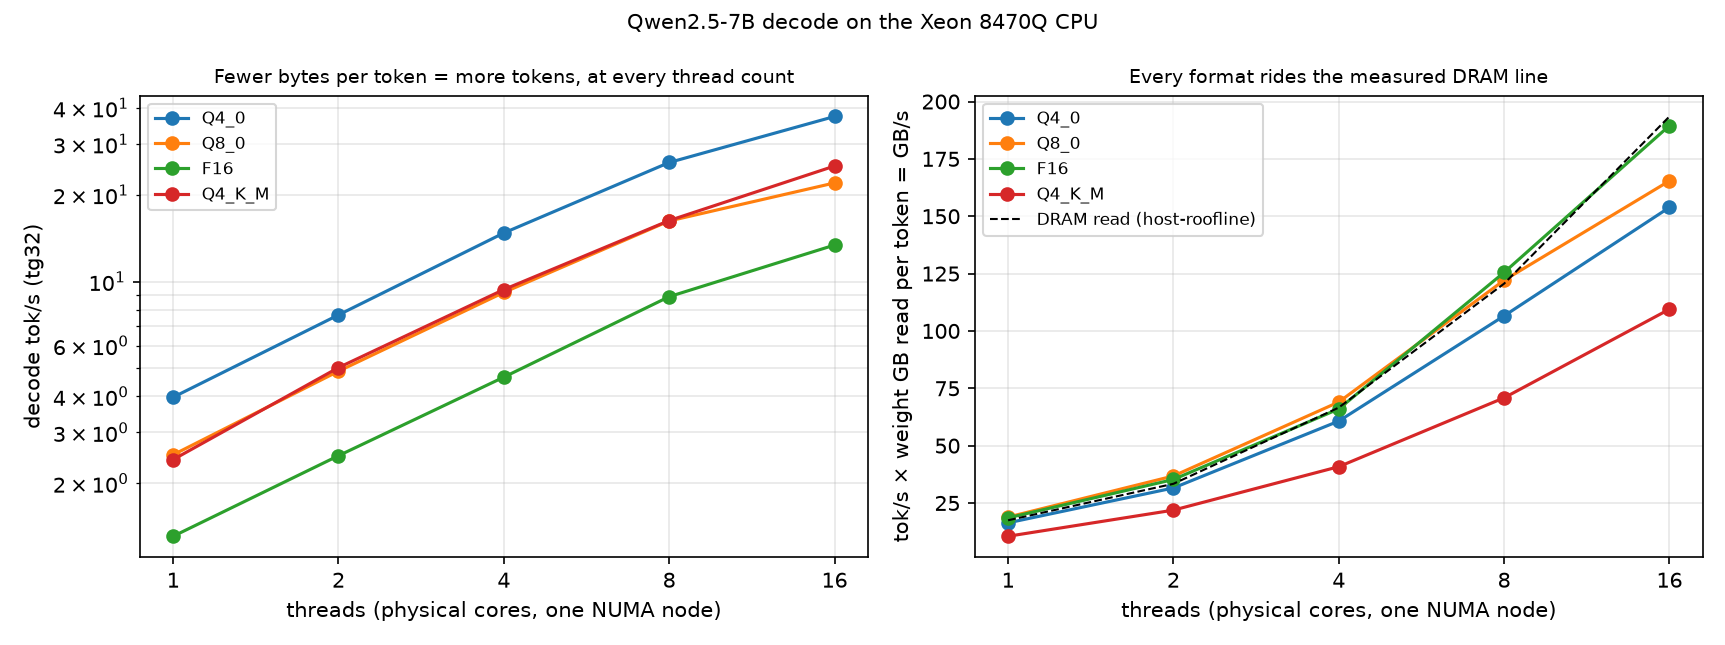
\includegraphics[width=\linewidth]{cpu_decode.png}
\caption{Qwen2.5-7B 在 Xeon 上的解码。左：tok/s 随线程数；右：tok/s × 每 token 字节，与 host-roofline 实测的 DRAM 读带宽（虚线）对比。}\label{fig:cpu}
\end{figure}

Q4\_0 单线程 3.97 tok/s，乘以每 token 4.1 GB 是 16.3 GB/s，单核 DRAM 读的 93\%；16 线程 37.4 tok/s（154 GB/s）。
F16 在 16 线程 13.4 tok/s，189 GB/s，几乎是 DRAM 读的全部。单线程解码测的就是单核的带宽：单核能挂起的 cache miss 有限，
带宽 = 在途字节 / 延迟（Little 定律），而不是总线宽度。这正是 roofline 模型~\cite{roofline} 里带宽那条斜线在单核上的含义。

\begin{table}[H]
\centering\small
\caption{CPU 上每种格式离带宽线多远（16 线程，tg32）}\label{tab:cpufmt}
\begin{tabular}{lrrrrr}
\toprule
格式 & 每 token GB & 1 线程 tok/s & 16 线程 tok/s & 16 线程 GB/s & 占 193.5 \\
\midrule
F16 & 14.15 & 1.31 & 13.4 & 189 & 98\% \\
Q8\_0 & 7.52 & 2.51 & 22.0 & 165 & 85\% \\
Q4\_0 & 4.12 & 3.97 & 37.4 & 154 & 79\% \\
Q4\_1 & 4.52 & 3.15 & 31.8 & 144 & 74\% \\
Q4\_K\_M & 4.34 & 2.42 & 25.2 & 109 & 56\% \\
Q3\_K\_M & 3.53 & 2.65 & 27.4 & 97 & 50\% \\
Q2\_K & 2.80 & 2.71 & 30.3 & 85 & 44\% \\
\bottomrule
\end{tabular}
\end{table}

\begin{findingbox}[：CPU 上更少的字节不等于更快]
Q2\_K 的字节是 Q4\_0 的 68\%，解码慢 19\%；Q4\_K\_M 只比 Q4\_0 多 5\% 字节，慢 33\%。
K-quant 每 256 个权重有两级 scale（超块 fp16 + 子块 6 bit 或 4 bit），解包要多做移位、取子块 scale、乘子块 scale，
这些整数指令在 CPU 上和点积争同一组向量端口，藏不进访存。简单格式（Q8\_0、Q4\_0、Q4\_1）每块一个 scale，而且能走 AMX 重排（\cref{sec:amx}），
到 DRAM 读的 74--85\%。这是由字节与速度的反常推出的，容器里没有 perf 权限，没有用计数器确认。
\end{findingbox}

\subsection{AMX 权重重排}\label{sec:amx}

\begin{table}[H]
\centering\small
\caption{\texttt{--repack 0/1}，16 线程，pp512 / tg64}\label{tab:repack}
\begin{tabular}{llrrr}
\toprule
格式 & 重排 & pp512 tok/s & tg64 tok/s & tg × 每 token GB \\
\midrule
Q4\_0 & 关 & 93.5 & 26.5 & 109 GB/s \\
Q4\_0 & 开（AMX） & 261.1 & 37.0 & 152 GB/s \\
Q8\_0 & 关 & 94.6 & 17.0 & 127 GB/s \\
Q8\_0 & 开（AMX） & 256.3 & 22.0 & 165 GB/s \\
\bottomrule
\end{tabular}
\end{table}

\texttt{-v} 日志里每个 Q4\_0 / Q8\_0 权重都有一行 \texttt{amx repack tensor}：加载时把权重排成 AMX tile 要的 VNNI 布局。
prefill 是大 M 的 GEMM，AMX 快 2.7--2.8 倍，与 int8-kernels lab 里 AMX 对 VNNI 打包的 3.0 倍同量级；解码是 M = 1 的 GEMV，tile 浪费 15/16 的行，
但重排后的连续布局减少了解包指令，解码快 1.3--1.4 倍，回到离 DRAM 读不远的 152--165 GB/s。
不重排时 Q4\_0（109 GB/s）比 Q8\_0（127）还低：每字节要做的解包更多，先撞上指令瓶颈——与 q4-gemv 里自写 Q4 内核的问题相同。

Q8\_0 不重排的 tg 第一次测到 $9.8\pm8.5$ tok/s：同一时间 5 个 ORT 任务把 cgroup 的 22 核配额挤满。标准差与均值同量级的点必须丢掉重跑，
表中数字来自单独重跑（$17.0\pm0.5$ 与 $22.0\pm0.2$）。

\begin{iqbox}{AMX 是很大的 int8 算力，为什么解码只快 1.3 倍？}
解码每 token 每个权重只用一次（2 FLOP 对 0.5--1 字节），算术强度只有每字节几个 FLOP，远低于 AMX 的拐点，是带宽受限。AMX 对解码的作用不是“多算”，
而是重排后解包指令变少，让解码从指令受限回到带宽受限：Q4\_0 从 109 GB/s 回到 152 GB/s，再往上就是 193.5 GB/s 的 DRAM 墙。
prefill 是 GEMM，才吃到 AMX 的算力，2.8 倍。
\end{iqbox}

\section{GPU：每种格式的速度}

\begin{figure}[H]
\centering
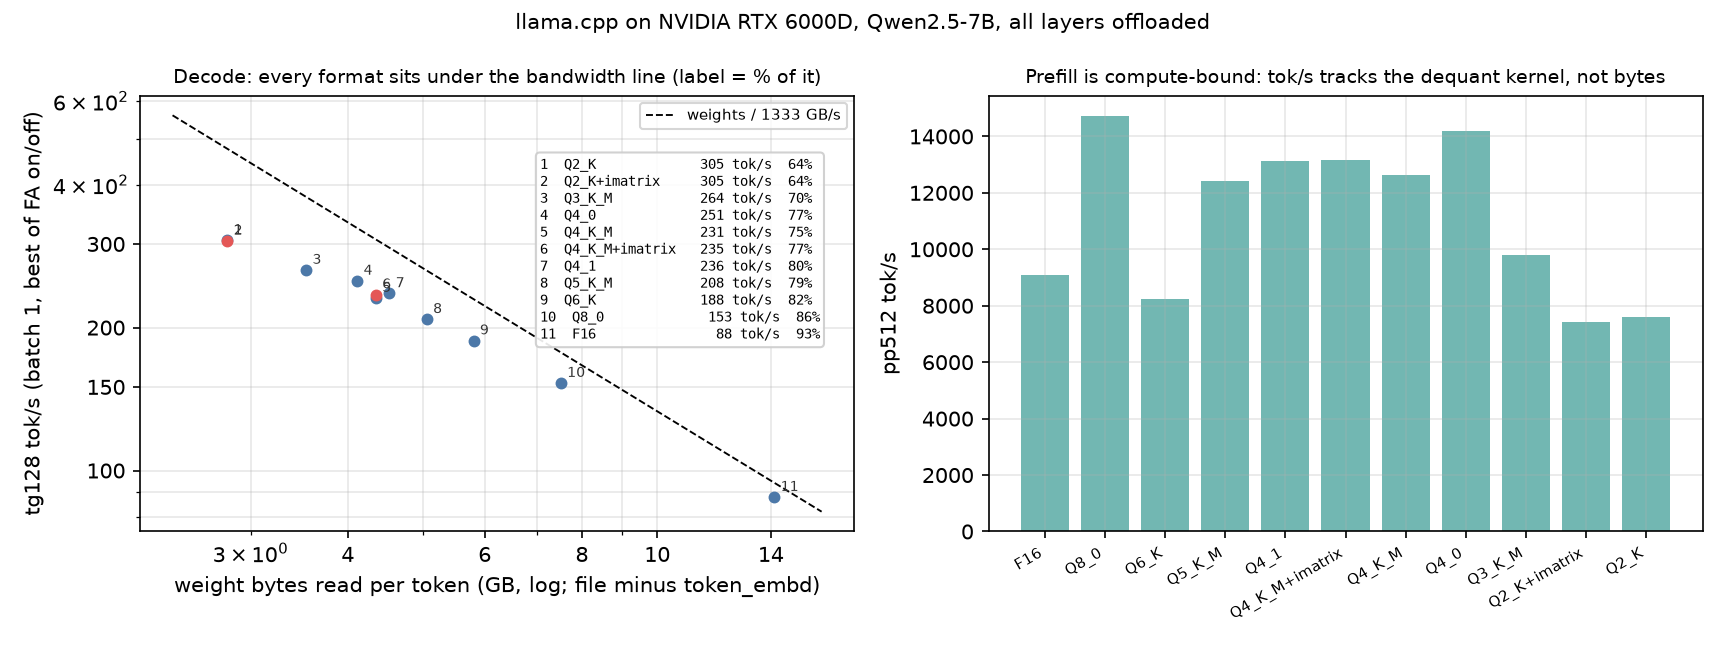
\includegraphics[width=\linewidth]{gpu_formats.png}
\caption{RTX 6000D，全部层 offload。左：解码 tok/s 对每 token 字节，虚线是 1333 GB/s 的字节上界，框中百分比是离上界多远；右：prefill。}\label{fig:gpu}
\end{figure}

\begin{figure}[H]
\centering
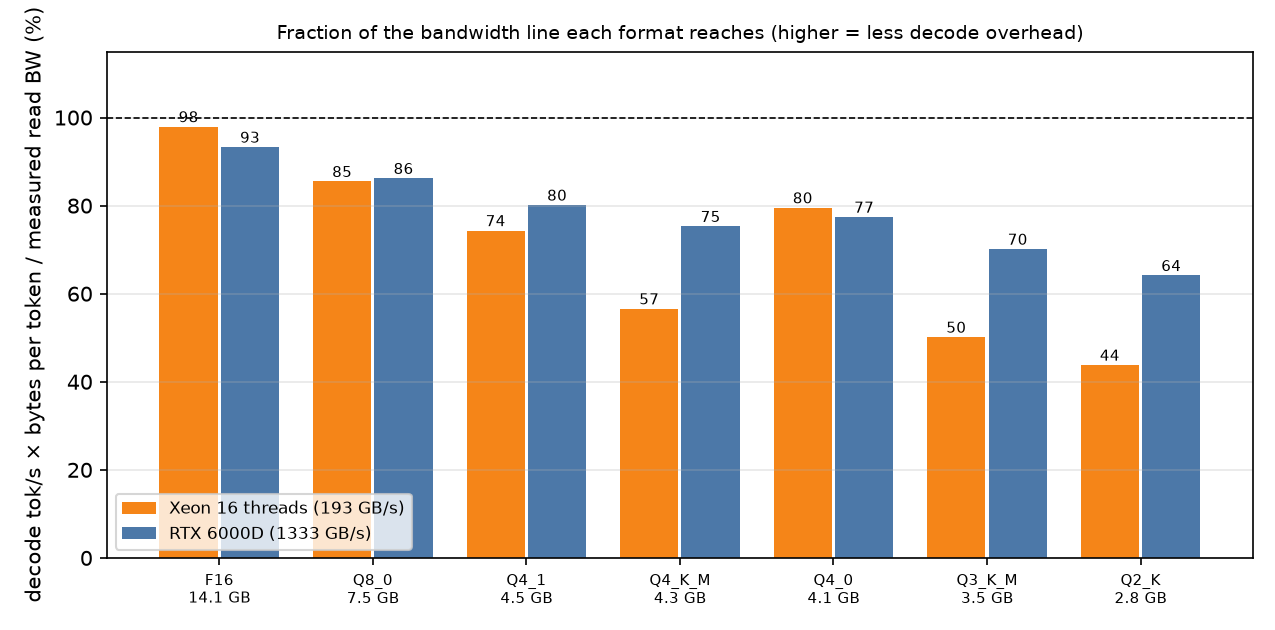
\includegraphics[width=0.85\linewidth]{bw_efficiency.png}
\caption{同一种格式在 CPU（16 线程）和 GPU 上离各自带宽线的距离。}\label{fig:eff}
\end{figure}

GPU 上解码同样按字节排序：F16 87.9、Q8\_0 152.8、Q4\_K\_M 230.7、Q4\_0 250.7、Q2\_K 305.3 tok/s；离带宽线的距离从 F16 的 93\% 降到 Q2\_K 的 64\%。
下降的原因是每 token 有一段不随权重字节变化的时间（\cref{sec:pred}）。\Cref{fig:eff} 是本报告的核心对比：
GPU 上 Q4\_K\_M（75\%）与 Q4\_0（77\%）几乎一样，CPU 上是 56\% 对 79\%。GPU 每字节可用的 ALU 多得多，K-quant 的解包被访存延迟藏住。

prefill 受算力限，速度由每种格式的“反量化 + matmul”内核决定，与字节无关：Q8\_0 14.7k、Q4\_0 14.2k tok/s 最快，Q6\_K 8.2k、Q2\_K 7.6k 最慢。

\section{质量：困惑度与 KL 散度}

\begin{figure}[H]
\centering
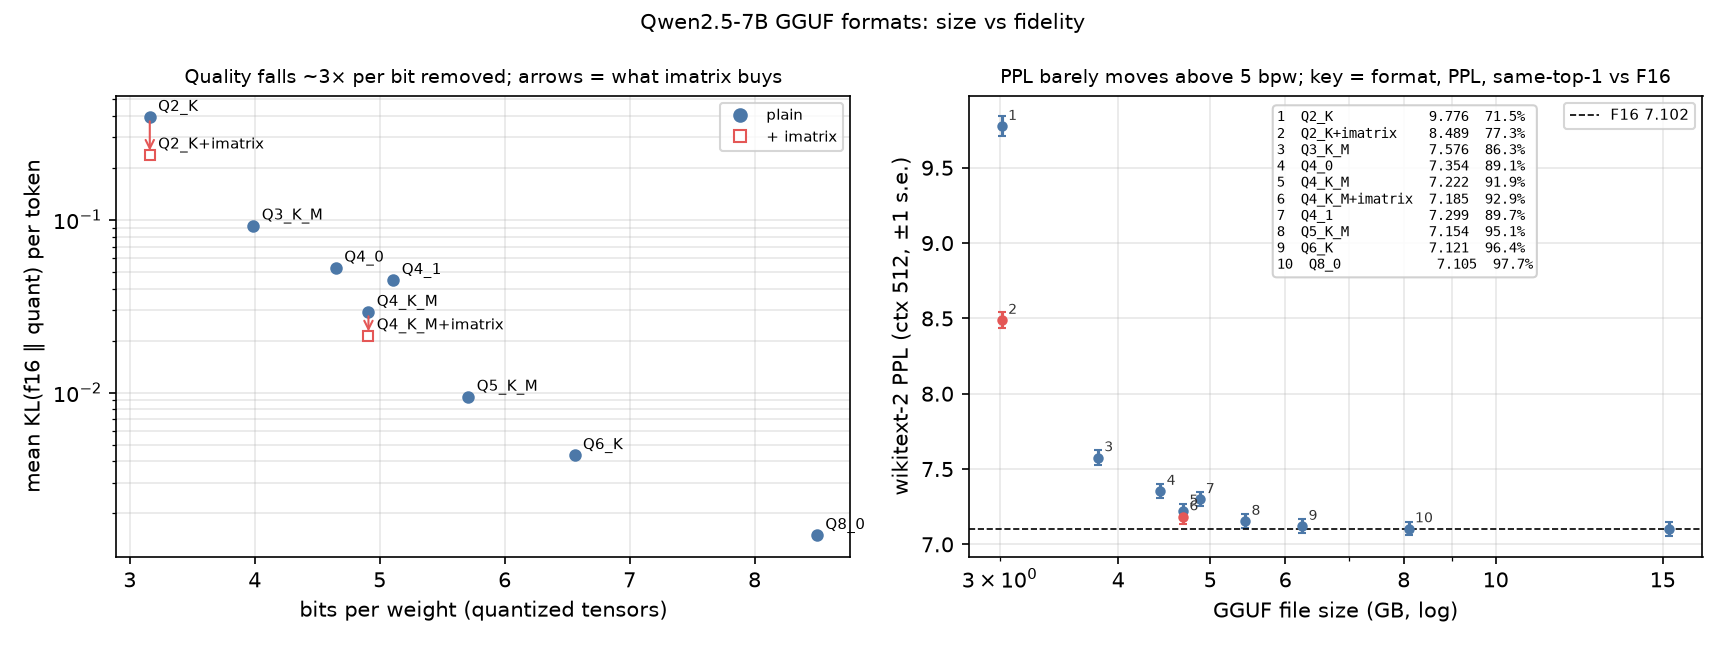
\includegraphics[width=\linewidth]{quality.png}
\caption{左：平均 KL(F16 ‖ 量化) 对 bpw，箭头是 imatrix 的收益；右：困惑度对文件大小，框中给出同 top-1 比例。}\label{fig:quality}
\end{figure}

\begin{table}[H]
\centering\small
\caption{质量（\texttt{quality.csv}）}\label{tab:quality}
\begin{tabular}{lrrrrr}
\toprule
格式 & bpw & PPL & 平均 KLD & KLD p99 & 同 top-1 \\
\midrule
F16 & 16 & 7.1016 & -- & -- & -- \\
Q8\_0 & 8.50 & 7.1052 & 0.0015 & 0.009 & 97.7\% \\
Q6\_K & 6.56 & 7.1207 & 0.0043 & 0.030 & 96.4\% \\
Q5\_K\_M & 5.71 & 7.1544 & 0.0094 & 0.082 & 95.1\% \\
Q4\_1 & 5.11 & 7.2990 & 0.0447 & 0.394 & 89.7\% \\
Q4\_K\_M & 4.91 & 7.2222 & 0.0292 & 0.271 & 91.9\% \\
Q4\_K\_M + imatrix & 4.91 & 7.1846 & 0.0214 & 0.221 & 92.9\% \\
Q4\_0 & 4.65 & 7.3537 & 0.0527 & 0.431 & 89.1\% \\
Q3\_K\_M & 3.99 & 7.5764 & 0.0923 & 0.805 & 86.3\% \\
Q2\_K & 3.16 & 9.7763 & 0.3925 & 2.483 & 71.5\% \\
Q2\_K + imatrix & 3.16 & 8.4893 & 0.2378 & 1.810 & 77.3\% \\
\bottomrule
\end{tabular}
\end{table}

\begin{itemize}
  \item KL 散度每少 1 bit 约涨 3 倍。困惑度很迟钝：Q8\_0 到 Q5\_K\_M 只从 7.105 涨到 7.154（+0.7\%），同 top-1 已从 97.7\% 掉到 95.1\%，
  即每 20 个 token 就有一个与 F16 选得不同。KLD 的 p99 比平均值更早报警。
  \item 同约 4.5 bpw，Q4\_K\_M 的 KLD 是 Q4\_0 的 0.55 倍；Q4\_1 更大却更差。K-quant 每 16--32 个权重有自己的步长，\texttt{\_M} 还对重要张量混用 Q6\_K。
  \item imatrix 是校准集上每个输入通道激活平方的均值，量化时按它给误差加权——和 AWQ~\cite{awq}、GPTQ~\cite{gptq} 同一个思想：误差要按激活加权。
  它在 Q4\_K\_M 上降 KLD 27\%，在 Q2\_K 上降 39\%、把 PPL 从 9.78 拉回 8.49；只改变选哪个量化值，不改变存储，速度相同。
\end{itemize}

\begin{iqbox}{端侧 CPU 和 GPU 服务器上，7B 模型分别选哪个 4-bit 格式？}
GPU 上选 Q4\_K\_M（+ imatrix）：解码只比 Q4\_0 慢 8\%，KL 散度低 45--60\%。CPU 上要看是否受指令限：在这台 Xeon 上 Q4\_0 解码快 1.48 倍（AMX 重排 + 解包简单），
代价是 1.8 倍的 KL 散度；如果质量要求高，Q5\_K\_M 或 Q4\_K\_M 更合适，但要接受 CPU 只能用到 50--60\% 带宽。
结论依赖“每字节有多少 ALU”：在更弱的端侧 CPU（如 Cortex-A76）上，指令受限会更严重，Q4\_0 的优势更大。
\end{iqbox}

\section{batch：吞吐与每路速度}

\begin{figure}[H]
\centering
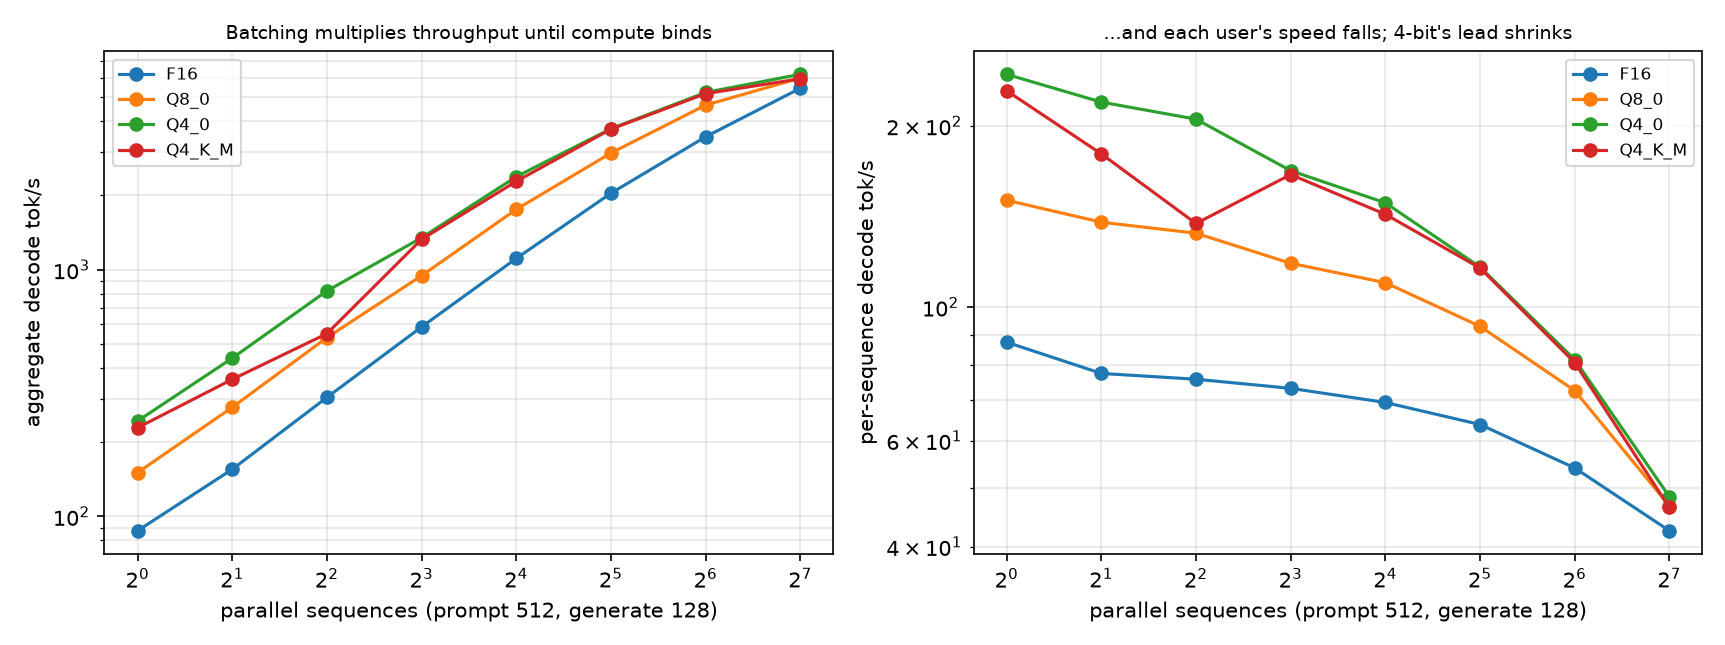
\includegraphics[width=\linewidth]{batched.png}
\caption{\texttt{llama-batched-bench}，prompt 512 + 生成 128，FA 开。左：聚合解码吞吐；右：每路解码速度。}\label{fig:batched}
\end{figure}

\begin{table}[H]
\centering\small
\caption{聚合解码 tok/s}\label{tab:batched}
\begin{tabular}{rrrrrr}
\toprule
并发 & F16 & Q8\_0 & Q4\_0 & Q4\_K\_M & Q4\_0 每路 \\
\midrule
1 & 87 & 150 & 244 & 229 & 243.5 \\
4 & 304 & 531 & 821 & 551 & 205.1 \\
16 & 1111 & 1756 & 2383 & 2281 & 149.0 \\
64 & 3459 & 4649 & 5234 & 5175 & 81.8 \\
128 & 5441 & 5985 & 6198 & 5948 & 48.4 \\
\bottomrule
\end{tabular}
\end{table}

1 路时 Q4\_0 是 F16 的 2.8 倍，128 路时只有 1.14 倍：每读一遍权重被 128 个序列分摊，瓶颈变成算力和 KV cache 的读取，四种格式收敛到 5.4--6.2k tok/s。
F16 聚合吞吐涨 62 倍、Q4\_0 只涨 25 倍——越受带宽限的配置，批处理收益越大。Q4\_K\_M 在 2--4 路时每路速度比 8 路还低（179.6、137.6 对 166.0），
llama.cpp 对小 batch 的量化 matmul 按 batch 大小切换内核，这一段 K-quant 选的路径不划算；没有逐个内核 profile。

\begin{iqbox}{量化在服务端还值得做吗？}
看工作点。低并发（交互式、端侧）下解码受带宽限，Q4 直接带来 2.5--2.8 倍；高并发下受算力限，权重字节不再是瓶颈，Q4 对 F16 只剩 1.14 倍，
这时量化的价值是省显存（放更多 KV cache、更大 batch），而不是每步更快。要在高并发下继续加速，需要 W8A8 / FP8 这类让 GEMM 本身变快的量化。
\end{iqbox}

\section{和 q4-gemv 的预测对照}\label{sec:pred}

\begin{table}[H]
\centering\small
\caption{q4-gemv 只算 196 个 Linear（CUDA graph）的预测 vs llama.cpp 端到端，同一张 RTX 6000D}\label{tab:pred}
\begin{tabular}{lrrrr}
\toprule
格式 & 预测 tok/s & 实测 tok/s & 比值 & 每 token 时间差 \\
\midrule
fp16 / F16 & 91.7（10.91 ms） & 87.9（11.38 ms） & 0.96 & 0.47 ms \\
Q8 / Q8\_0 & 163.0（6.13 ms） & 152.8（6.54 ms） & 0.94 & 0.41 ms \\
Q4\_0 & 283.7（3.52 ms） & 250.7（3.99 ms） & 0.88 & 0.46 ms \\
\bottomrule
\end{tabular}
\end{table}

\begin{findingbox}[：层时间之和只差一个常数项]
三种格式的端到端解码都比只算 Linear 的预测多 0.41--0.47 ms/token，与权重字节无关。这是 Linear 以外的每 token 固定成本：28 层的 attention、
RMSNorm、RoPE、残差、采样与 llama.cpp 的图调度。q4-gemv 的模型在结构上是对的，缺的是这个常数；权重越小它占比越大
（F16 4\%，Q4\_0 12\%），也正是 GPU 上带宽线百分比随格式下降的原因。要让 Q4 解码更快，下一步优化的是这 0.45 ms，而不是 GEMV 内核。
\end{findingbox}

\begin{caveatbox}
\begin{itemize}
  \item CPU 数字来自 cgroup 限 22 核、宿主有其他租户的容器；被限流的点已剔除重跑，但不能排除残留噪声。
  \item 每 token 字节是估算：没扣 KV cache 的读取，也没区分 output.weight 与其他张量的类型。
  \item 困惑度协议是 llama-perplexity 的 ctx 512，与 mlsys-infra compiler-compression 的 HF ctx 1024 协议不同，不能直接比较。
  \item Q2\_K + imatrix 的量化日志没有落盘，其 bpw 取自 Q2\_K（imatrix 不改变布局，两文件只差 224 字节元数据）。
  \item 0.45 ms 的固定成本没有用 nsys 拆到具体算子；CPU 上“指令受限”的判断没有计数器证据。
\end{itemize}
\end{caveatbox}

\section{复现}

\begin{lstlisting}[language=bash]
cd solutions/edge-runtime/llama-cpp-7b
python -m pytest -q tests
python scripts/run_experiments.py prep cpu        # f16 GGUF, Q8_0 / Q4_0, llama-bench 1..16 threads
python scripts/run_experiments.py gpu batched     # imatrix, KLD base, per format quantize -> bench -> PPL -> KLD
python scripts/run_experiments.py summarize       # tables and figures from artifacts/raw only
\end{lstlisting}

路径由环境变量给出（\texttt{LLAMA\_CPP}、\texttt{HF\_MODEL}、\texttt{GGUF\_WORK}、\texttt{GGUF\_QDIR}、\texttt{CPU\_CORES} 等）；
原始数据在 \nolinkurl{solutions/edge-runtime/llama-cpp-7b/artifacts/raw/}。

\begin{thebibliography}{99}
\bibitem{llamacpp} G. Gerganov et al. llama.cpp: LLM inference in C/C++. \url{https://github.com/ggml-org/llama.cpp}, commit \texttt{149f564}, 2026.
\bibitem{qwen25} Qwen Team. Qwen2.5 Technical Report. arXiv:2412.15115, 2024.
\bibitem{wikitext} S. Merity, C. Xiong, J. Bradbury, R. Socher. Pointer Sentinel Mixture Models. In \emph{ICLR}, 2017.
\bibitem{roofline} S. Williams, A. Waterman, D. Patterson. Roofline: An Insightful Visual Performance Model for Multicore Architectures. \emph{Communications of the ACM}, 52(4), 2009.
\bibitem{gptq} E. Frantar, S. Ashkboos, T. Hoefler, D. Alistarh. GPTQ: Accurate Post-Training Quantization for Generative Pre-trained Transformers. In \emph{ICLR}, 2023.
\bibitem{awq} J. Lin, J. Tang, H. Tang, S. Yang, W.-M. Chen, W.-C. Wang, G. Xiao, X. Dang, C. Gan, S. Han. AWQ: Activation-aware Weight Quantization for LLM Compression and Acceleration. In \emph{MLSys}, 2024.
\end{thebibliography}

\end{document}
